
%(BEGIN_QUESTION)
% Copyright 2010, Tony R. Kuphaldt, released under the Creative Commons Attribution License (v 1.0)
% This means you may do almost anything with this work of mine, so long as you give me proper credit

Calculate the following parameters in this 3-wire RTD circuit, assuming an RTD temperature of 174 $^{o}$F and $\alpha = 0.00385$ $\Omega$/$\Omega$/$^{o}$C:

$$\includegraphics[width=15.5cm]{i00668x01.eps}$$

\begin{itemize}
\item{} $V_{out}$ = \underbar{\hskip 50pt} millivolts
\vskip 10pt
\item{} $V_{AD}$ = \underbar{\hskip 50pt} millivolts 
\vskip 10pt
\item{} $V_{AB}$ = \underbar{\hskip 50pt} millivolts 
\vskip 10pt
\item{} $V_{CB}$ = \underbar{\hskip 50pt} millivolts 
\vskip 10pt
\item{} $V_{CF}$ = \underbar{\hskip 50pt} millivolts 
\end{itemize}

Note: you need only to state voltage magnitudes, not polarities, in your answers.

\underbar{file i00668}
%(END_QUESTION)





%(BEGIN_ANSWER)

\begin{itemize}
\item{} $V_{out}$ = {\bf 32.59} millivolts (formula) \hskip 30pt {\bf 32.6175} millivolts (table) 
\vskip 10pt
\item{} $V_{AD}$ = {\bf 32.59} millivolts \hskip 30pt {\bf 32.6175} millivolts (table) 
\vskip 10pt
\item{} $V_{AB}$ = {\bf 0} millivolts 
\vskip 10pt
\item{} $V_{CB}$ = {\bf 0.25} millivolts 
\vskip 10pt
\item{} $V_{CF}$ = {\bf 0.25} millivolts 
\end{itemize}

%(END_ANSWER)





%(BEGIN_NOTES)

{\bf This question is intended for exams only and not worksheets!}.

%(END_NOTES)

